\def\theTopic{Correlation/Slope }
\def\dayNum{17 }

\begin{center}

{\bf {\large Who Looks Good to You?}}
\end{center}


Christian Rudder works for the dating web site OKcupid, and has
written a book, {\it Dataclysm} about some surprising data 
collected from the web site.

As an example, here are plots he gives for women and for men.
The horizontal axis is the age of the man or woman being
interviewed. The vertical axis is the age which they think looks most
attractive in the opposite sex.\vspace{-.5cm}

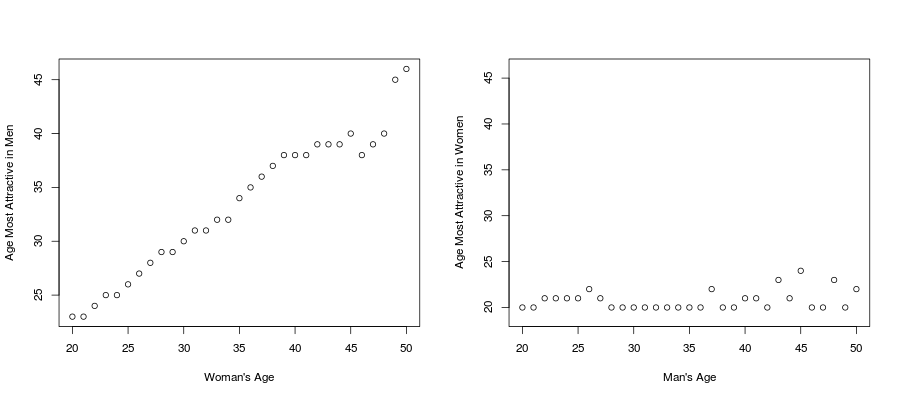
\includegraphics[width=\linewidth]{../plots/attractiveAges.png}

There are clearly big differences between men and women, so we want to
describe them with statistics.\vspace{-.5cm}
\begin{enumerate}
  \item Suppose you're talking to a friend over the telephone, and
    you need to explain  that the same two variables
    have a different relationship for women than for men. How would you
    describe the two plots? 
\begin{students}
 \vspace{2cm}      
\end{students}

\begin{key}
  {\it  I'm hoping for some talk about fitting a line or about slope
    or correlation.}
\end{key}

\item What statistical summaries differ in the two plots?
\begin{students}
 \vspace{2cm}      
\end{students}

\begin{key}
  {\it  Means of the y variable certainly differ,  but again I hope
    they think of slope  or correlation. }
\end{key}



\item As a review, in Algebra class you would have learned an equation
  for a linear relationship between $x$ and $y$.  What letters did you
  use for slope and intercept?  What does ``slope'' mean?  What does
  ``intercept'' mean?
\begin{students}
 \vspace{2cm}      
\end{students}

\begin{key}
  {\it $m$ for slope = rise over run?, $b$ for intercept = $y$ value
    when $x=0$. Other answers are possible.}
\end{key}


  In Statistics, we use the following equation for a ``true'' regression  line:
  $$ y = \beta_0 + \beta_1 x + \epsilon  $$
  and when we estimate the line we add hats to the parameters,
  $\beta_0$ and $\beta_1$, and also to the left side to say we have an
  estimated response, $\hat{y}$.
  $$ \hat{y} = \hat{\beta}_0 + \hat{\beta}_1 x$$
\item Take a guess at the  slopes for the two plots above.
\begin{students}
 \vspace{2cm}      
\end{students}

\begin{key}
  {\it Women: less than one -- perhaps .75?  Men: slightly bigger than
    zero, like 1/30?  }
\end{key}

  \item {\bf Correlation} measures the strength and direction of a {\bf
  linear} relationship between two quantitative variables. It is a
unit-less number between -1 and 1 with zero meaning ``uncorrelated'' and
1 or -1 meaning perfect correlation -- points fall right on a
line. The sample correlation is called $r$, and the true correlation
is $\rho$, the Greek letter ``rho''. 
 The sign  of the correlation tells us if the one variable
 increases as the other does (positive) or decreases (negative).

   Go to  \url{http://www.tylervigen.com/ } and find a
    ``spurious'' correlation which has correlation coefficient, $r$ less
    than -0.90 and one that has $r > 0.99$.  Here are the two
    variables plotted without year ( a lurking variable).\\
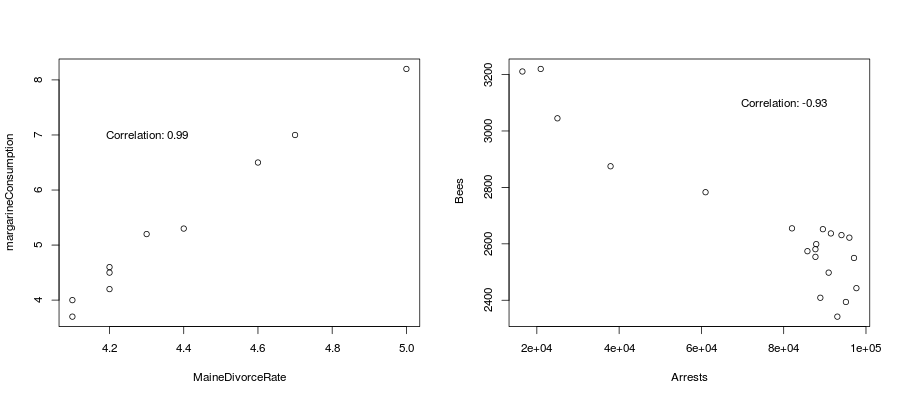
\includegraphics[width=\linewidth]{../plots/spuriousCorr.png}
    The point here is that if you search through lots of variables,
    you can find pairs that increase in the same way, or oppositely.

    Just to show you found the site, what variables are in the first
    plot, and what is their correlation?
\begin{students}
 \vspace{1cm}      
\end{students}

\begin{key}
  {\it  US spending on Science, Space, Technology has correlation 0.99
  with Suicides by hanging, suffocation, and drowning.}
\end{key}

\item Why are the values on that page called ``spurious''?
\begin{students}
 \vspace{1cm}      
\end{students}

\begin{key}
  {\it Because there is no reason that the two variables should be
    correlated. }
\end{key}

\item Correlations in the following plot are either 0.96 or 0.56.
  Which is which?\\
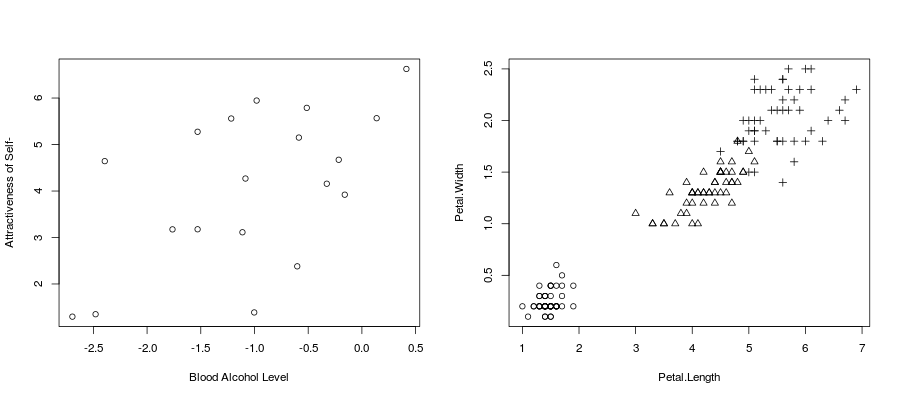
\includegraphics[width=\linewidth]{../plots/realCorr.png}
\begin{students}
 \vspace{1cm}      
\end{students}

\begin{key}
  {\it 0.56 - attractiveness and BAL, and 0.96 - petals}
\end{key}

  The first is data recreated from summary stats given for a study of
  how attractive men felt they were and their blood alcohol level (log
  scale, so negative numbers do make sense).
  The second shows measurements of iris petals. The clusters are for
  three different species. Within
  species correlations are quite different: 0.33, 0.79 and 0.32, but
  with all the data, correlation is higher. 

\item Look back at the Age-Attraction plots from OKcupid.
  Guess what those correlations are for women and for men.
\begin{students}
 \vspace{1cm}
\end{students}

\begin{key}
  {\it 0.98  and 0.28}
\end{key}

\item Correlation contest:\\
  Go to
  \url{http://www.rossmanchance.com/applets/GuessCorrelation.html}.
  Click \fbox{$\surd$} {\sf Track Performance}, then each member of your
  group guesses correlation for 5 \fbox{New Sample}s. (Click \fbox{\sf
    Reset} between each person.)  The first plot
  below {\sf Track Performance} tells you the correlation between your
  guesses and the true values.  What  is it? What's the best one in
  your group? 
\begin{students} 
\vspace{1cm}
\end{students}



\begin{center}
  {\bf Slope}
\end{center}

\item  In Algebra, a line is a collection of points satisfying an
     equation. In Statistics we start with data and have to find a good
     line to represent the relationship between two variables.  When
     there is a lot of scatter in the points, many lines look
     reasonable.  Go to 
     \url{http://www.rossmanchance.com/applets/RegShuffle.htm}
     to see data on people's foot length versus height.
     \begin{enumerate}
     \item Is this a linear relationship? \\
     \item Positive or Negative? \\
     \item Strong, Moderate, or Weak? \\
     \item Guess the correlation, then check with the button below the
       plot.
     \end{enumerate}
\begin{key}
 Linear, positive, moderately strong.      $ r = .71$  
\end{key}

   We'll use this app for the rest of this activity.

\item Click {\sf Show Movable Line:} \fbox{$\surd$} and move the
  center by dragging the large green square in the middle and adjust
  the slope by dragging either end of the line up or down.  Get the
  line which you think best fits, write its equation here:
  $$ \widehat{\mbox{height}} = \_\_\_\_ + \_\_\_\_ \times \mbox{footlength}$$
\begin{students}
 \vspace{.2cm}      
\end{students}

\begin{key}
  {\it I got intercept 40.5, slope = 0.94}
\end{key}
\item Click {\sf Show Regression Line:} \fbox{$\surd$} and write the
  equation here:
  $$ \widehat{\mbox{height}} = \_\_\_ + \_\_\_ \times
  \mbox{footlength}$$
\begin{key}
  {\it $ \widehat{y} = 38.3 + 1.03 x$}
\end{key}
\begin{enumerate}
  \item Was your slope too large? too small? about right? 

  \item What height does this line give for a person whose foot length
    is 0?\vspace{.9cm}\\

    (This is an example of {\bf extrapolation}: predicting $y$ for an $x$ value
    outside the range of observed $x$'s.)
\end{enumerate}


\item  Let's see how much we can change slope and correlation by
  adding just one more point.  Give it a new ``x''  value of 60 cm.
  Pick a ``y'' value which you think will change the general pattern
  we see between length and height. Can you get the correlation to go
  close to zero?  I'm not having luck with ``move observations'' but
  you can edit the last line of data to try  new ``y'' values  until
  you get a correlation of about zero.  
  \begin{enumerate}
  \item 
  What are the coordinates of
  the added point?
\begin{students}
 \vspace{1cm}      
\end{students}

\begin{key}
  {\it (50, 56.4) has $r = 0.001$}
\end{key}
\item 
  Now what is the slope of the regression line? 
\begin{students}
 \vspace{1cm}      
\end{students}

\begin{key}
  {\it Close to 0 as well, I got a weird underflow problem, but it's
    about 0.0009}
\end{key}
\item Is correlation resistant to outliers?  Is slope? Explain.
  \begin{students}
 \vspace{1cm}      
\end{students}
\begin{key}
  {\it No.  One outlier completely changed correlation and slope.}
\end{key}
\end{enumerate}
\item Click \fbox{\sf Revert} to go back to the original data. Have it
  show the regression line and the residuals.  You can't see from the
  plot, but points below the line have negative residuals, points
  above the line have positive residuals according to this definition:
$$ \mbox{residual} = \mbox{observed} - \mbox{predicted or } 
       e = y - \hat{y}$$
 \begin{enumerate}
   \item   Which residual is largest?
     Find the (x, y) pair  in the data table associated with that
     point.
\begin{students}
 \vspace{1cm}      
\end{students}

\begin{key}
  {\it (30, 74)}
\end{key}
\item Compute it's predicted value using the equation given.  Also
     compute the residual for the one furthest below the line.
\begin{students}
 \vspace{1cm}      
\end{students}

\begin{key}
  {\it (30, 74) has the largest residual of $74 - (38.3 +1.03\times
    30) = 74 - 69.2 = 4.8$.   Smallest comes from (24, 56) with
    predicted value $38.3+1.03\times 24 = 63.02$ so its residual is
    $56 - 63.02 = -7.02$ }
\end{key}
   \item Now click {\sf Show Squared Residuals}.  These are important
     because we are using the ``Least Squares'' line. It picks slope
     and intercept to minimize the sum of all the squared residuals.
     Write down SSE (sum of squared errors). 
\begin{students}
 \vspace{1cm}      
\end{students}

\begin{key}
  {\it 235}
\end{key} 
Any other line will have larger SSE.
\end{enumerate}
\end{enumerate}

\begin{center}
  {\bf Take Home Messages:}\vspace{-.4cm}
\end{center}
\begin{itemize}
\item It's not right to speak of the correlation between gender (or any
  categorical variable) and age, or between two categorical variables.
\item It only works for linear relationships.  We can have very strong
  nonlinear association with correlation near zero.
\item Positive relationships mean large values in one variable are
  generally  paired  with large values  in  the other variable
  (and small with small).  Negative relationships pair large with small.
\item Correlation has no units and is restricted to the interval
  (-1,1). Both end of the interval indicate very strong
  correlation. Near zero, we say the two variables are uncorrelated.

\item Neither correlation nor slope are resistant to outliers.  A
  change in one point can completely change these values.
\item Slope of the ``Least Squares'' line is given the label
  $\hat{\beta}_1$ because it estimates the true slope, $\beta_1$.  It is
  related to correlation.  
  $$  \hat{\beta}_1 = r \times\frac{s_y}{s_x}$$
  where $s_y$ is the Standard Deviation (SD) of the responses, and $s_x$ is
  the SD of the explanatory variable.
\end{itemize}



